%-------------------------------------------------------------------------------
\section{Data Disguising}
%-------------------------------------------------------------------------------
\begin{figure}[t!]
    \centering
    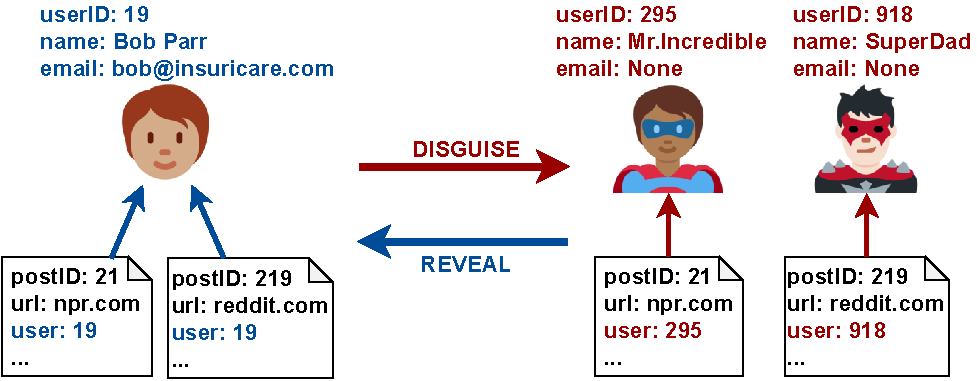
\includegraphics[width=0.47\textwidth]{img/disguises_new}

    \caption{Disguises move the target object (in this example, a user Bob) from an identity-revealing
    guise to privacy-preserving guises.}
    \label{fig:example}
\end{figure}

\ms{dumped some text here, will edit}
To solve these challenges, we propose \emph{data disguising}, a systematic approach to privacy
transformations. Data disguising reasons about \emph{disguises}, namely privacy transformations that
follow an organized structure and perform a restricted set of actions (\S\ref{sec:disguises}).
The structured nature of disguises allows a data disguising tool to automatically determine how to correctly
compose multiple disguises, and to check that the end-state achieves the desired privacy properties.
The tool uses the abstraction of \emph{per-user vaults}, which allow the tool to
reintroduce destroyed data from prior disguises as necessary, while still ensuring that user data
remains protected (\S\ref{sec:composition}).

A data disguising tool sits alongside the application database, and exposes an API to the
application allowing it to invoke disguises when necessary. Developers only need to determine when
to invoke the tool's API, and to provide the (necessarily application-specific) schema annotations
that describe each disguise; the tool then performs the necessary physical modifications to the application's
database to transform data as necessary.

\ms{old text follows}

Data disguising offers a systematic technique to tackle the complexity and challenges of performing
privacy transformations.
%
The key idea behind data disguising is to associate multiple \emph{guises} with a target data
object (\ie a row in a relational database). Guises vary in how they reveal identities or preserve privacy.
%
Objects move between different guises by means of disguises---a set of constrained privacy
transformations.

Figure~\ref{fig:example} illustrates this with the example of user account deletion.
%
When his account is active, user Bob's profile is associated with his true identity and all his
contributions to the site (an identity-revealing guise).
%
When Bob deletes his account, his profile and contributions move to different, privacy-preserving
guises: his name has been anonymized, his email address has been redacted, and his contributions
have been decorrelated and attributed to individual, unidentified user guises.
%
Decorrelation makes it seem as if a different user provided each of Bob's contributions. This allows
these contributions to be retained, while preventing an observer from correlating these
contributions back to Bob's identity, and while preserving referential integrity.

Disguises transform a guise by modifying it at per-attribute (\ie per-column) granularity, or
splitting it into multiple guises in order to decorrelating from objects that reference it (via \eg foreign-key relationships).
Guises can also be removed entirely.
At any given moment, an application's data comprises a mix of identity-revealing guises
and privacy-preserving ones. Disguises modify, split, and/or combine individual guises when triggered.

\subsection{Writing Disguises}
\label{sec:disguises}
The application developer writes a disguise specification for each privacy transformation needed
in the application.
%
When writing a disguise, developers can reason about its
specification in isolation; interactions between different disguises are handled by a disguising
tool (\S\ref{sec:composition}).
%
We assume that:
\begin{enumerate}[nosep]
  \item developers use their domain knowledge to write correct and complete disguises;
    %\lyt{a bit worried about ``complete'' here}
  \item application code handles the different guises appropriately (\eg in
    displaying them); and
  \item different guises of the same object have the same structure (\eg they can be
    rows in the same table).
\end{enumerate}
%
A data disguising tool takes a disguise specification and turns it into storage operations that
achieve the desired application data state.

Developers specify predicated transformations, which describes a disguised end-state of all
objects satisfying the predicate. For
example, Figure~\ref{fig:example} would include a specification that all email addresses be obfuscated in an anonymous manner for the user with name ``Bob Parr''.
%
Transformations can either remove objects, or change objects into one or more guises.
To create a guise from an object, developers specify how to transform attributes of the
object (\eg table column values) into guise attributes (\eg changing email addresses).

\iffalse
Developers choose how to create other guise attributes, selecting from among the following:
%
\paragraph{(1) Copy object content.}
%
Guises of the same object all share the object's attribute values.
%
If the attribute is a reference attribute (\eg a foreign key column), all guises will refer to the same object.
%
%
Copying allows developers to retain the object's content, without worrying about how to
synthesize attribute values for guises.
%
%However, this should only be chosen if guise attribute
%values cannot be generated, or if this attribute says little about the true identity of the
%entity.
For example, in Figure~\ref{fig:guises} the \texttt{darkmode} attribute is copied in
all guises.
%; the \texttt{darkmode} attribute reveals very little about the underlying user's
%identity.

\paragraph{(2) Generate new content.}
%
To create new attributes, developers specify whether the guise's value should be random,
a default value, or generated from the object's attribute value via a custom function (\eg hashing
the value).
%
Figure~\ref{fig:guises} illustrates an example of random (\texttt{name}) and default
(\texttt{active}) generated value attributes.
%
%
Creating new guise reference attributes (\eg new foreign key relationships) requires
creating a new guise for the referenced object in order to maintain referential
integrity;
the data disguise rewrites the reference to point to the new guise.
%
In Figure~\ref{fig:guises}, creating two user guises requires creating two
tag guises, and the tag guises' identifiers become the user guises' foreign keys.
%

\paragraph{(3) Copy object content, but only once.}
%
One guise copies the attribute value from the object, but all other guises generate new
values (as described above).
%
\texttt{notifs} in Figure~\ref{fig:guises} illustrates how the attribute is copied once.
%
This enables the application to retain the original object semantics (\eg a count of how many
users want notifications) without creating duplicates.
%
\begin{figure*}[t!]
    \centering
    \footnotesize
\begin{tabular}{@{}c|c|c|c@{}}
\textbf{User Transformation Spec} & \textbf{User Object} & \textbf{Guise 1} &
    \textbf{Guise 2} \\
\begin{lstlisting}[language=Rust]
"id":       IDAttribute,
"name":     Gen(Random),
"active":   Gen(Default(false)),
"darkmode": CopyAll,
"notifs":   CopyOnce+Gen(Default(false)),
"tag_id":   GenForeignKey,
\end{lstlisting}
    &
\begin{lstlisting}[language=Rust]
"id":       19,
"name":     BobParr,
"active":   true,
"darkmode": false,
"notifs":   true,
"tag_id":   11
\end{lstlisting}
&
\begin{lstlisting}[language=Rust]
"id":       295,
"name":     MrIncredible,
"active":   false,
"darkmode": false,
"notifs":   true,
"tag_id":   81483
\end{lstlisting}
&
\begin{lstlisting}[language=Rust]
"id":       918,
"name":     SuperDad,
"active":   false,
"darkmode": false,
"notifs":   false,
"tag_id":   15592
\end{lstlisting}
\end{tabular}
    \caption{Creating two guises of an example user (of a synthetic application schema).}
    \label{fig:guises}
\end{figure*}

\fi
